\documentclass[a4paper, 11pt, oneside]{report}

% Overleaf: set the main document to report.tex, then compile with pdfLaTeX.
% Copy "iiit manipur.png" from the format zip into figures/iiitmanipur.png.
% Optional screenshots, also under figures/:
%   depth.png  forecast.png  chat.png  tracker.png  photo-named.png  photo-withheld.png
% Change CSXXXX, the month, and the declaration date if the course notice differs.
% The internship offer-letter page from the format zip is omitted: this is a project report.

\usepackage{graphicx}
\usepackage{float}
\usepackage[table,xcdraw]{xcolor}
\usepackage[utf8]{inputenc}
\usepackage[T1]{fontenc}
\usepackage{fouriernc}
\usepackage{subcaption}
\usepackage{tikz}
\usetikzlibrary{arrows.meta, positioning, fit}
\usepackage{pgfplots}
\pgfplotsset{compat=1.18}
\usepackage{longtable}
\usepackage[nottoc]{tocbibind}
\usepackage{url}
\usepackage{amsmath}
\usepackage{booktabs}
\usepackage{array}
\usepackage{enumitem}
\usepackage{hyperref}

\hypersetup{
    colorlinks=true,
    linkcolor=black,
    citecolor=black,
    urlcolor=blue
}

\newcommand{\includelogo}[2][5cm]{%
    \IfFileExists{#2}{%
        \includegraphics[width=#1]{#2}%
    }{%
        \fbox{\parbox{#1}{\centering\vspace{8mm}Place the institute logo at\\ \texttt{#2}\vspace{8mm}}}%
    }%
}

\newcommand{\screenshot}[3]{%
    \begin{figure}[H]
        \centering
        \IfFileExists{#1}{%
            \includegraphics[width=0.92\textwidth]{#1}%
        }{%
            \fbox{\parbox{0.88\textwidth}{\centering\vspace{14mm}Screenshot to be inserted\\ \texttt{#1}\vspace{14mm}}}%
        }%
        \caption{#2}
        \label{#3}
    \end{figure}
}

\begin{document}

\begin{titlepage}
    \centering
    \vspace*{\baselineskip}
    \vspace{0.75\baselineskip}
    {\LARGE KrishiBee: A Machine-Learning Farm Advisory\\[0.4em] for Sowing Depth and Wheat Disease Screening}
    \vspace{0.75\baselineskip}
    \vspace{2\baselineskip}
    A report submitted for the course named Project-II (CSXXXX)
    \vspace*{5\baselineskip}
    Submitted By
    \vspace{0.5\baselineskip}
    {\scshape\Large Sourav Yadav\\ Semester~VII\\ 230101043\\ \normalsize sour230101043@iiitmanipur.ac.in}
    \vspace{0.5\baselineskip}
    Under the Guidance of
    \vspace{0.5\baselineskip}
    {\scshape\Large Dr.\ Rajkumari Bidyalakshmi Devi}
    \vspace{0.5\baselineskip}
    \vfill
    \begin{center}
        \includelogo{figures/iiitmanipur.png}
    \end{center}
    {\scshape\small Department of Computer Science and Engineering\\ Indian Institute of Information Technology Senapati, Manipur\\ November 2026}
\end{titlepage}

\begin{center}
    {\LARGE \textbf{Declaration}}
\end{center}

I hereby declare that the project work entitled ``KrishiBee: A Machine-Learning Farm Advisory for Sowing Depth and Wheat Disease Screening'' has been carried out by me under the supervision of Dr.\ Rajkumari Bidyalakshmi Devi, Assistant Professor, Department of Computer Science and Engineering, IIIT Senapati, Manipur.

In this submission, I have expressed my idea in my own words, and I have adequately cited and referenced any ideas or words that were taken from another source. I also declare that I adhere to all principles of academic honesty and integrity and that I have not misrepresented or falsified any ideas, data, facts, or sources in this submission. I affirm that this project report has not been submitted, either in part or in full, for the award of any other degree or diploma. If any violation of the above is made, I understand that the institute may take disciplinary action.

\vspace{1.2cm}
\hspace{7cm} Sourav Yadav \\
\vspace{0.4cm}
\hspace{7cm} 230101043 \\
\vspace{0.8cm}
\hspace{7cm} Date: 05-November-2026

\newpage

\begin{center}
    \thispagestyle{empty}
    \begin{table}
        \centering
        \includelogo[2.2cm]{figures/iiitmanipur.png}\\[0.4cm]
        \begin{tabular}{l}
            Department of Computer Science and Engineering \\
            Indian Institute of Information Technology Senapati, Manipur \\
        \end{tabular}
    \end{table}
    \par\noindent\rule{\textwidth}{0.4pt}

    Dr.\ Rajkumari Bidyalakshmi Devi
    \hspace*{\fill} Email: \href{mailto:bidyalakshmi@iiitmanipur.ac.in}{bidyalakshmi@iiitmanipur.ac.in}\\
    Assistant Professor
    \hspace*{\fill} Contact No: +91-7005126046\\[1.6cm]

    {\Huge \textbf{\emph{To Whom It May Concern}}}\\[1.4cm]

    \large
    This is to certify that the project report entitled \textbf{``KrishiBee: A Machine-Learning Farm Advisory for Sowing Depth and Wheat Disease Screening''}, submitted to the Department of Computer Science and Engineering, Indian Institute of Information Technology Senapati, Manipur, in partial fulfilment of the requirements for the award of the degree of Bachelor of Technology in Computer Science and Engineering, is a record of bona fide work carried out by \textbf{Sourav Yadav}, bearing roll number \textbf{230101043}.

    \vspace{1.6cm}
    \hspace*{2.4in} Signature of Faculty Advisor\\[0.3cm]
    \hspace*{2.3in} \textbf{(Dr.\ Rajkumari Bidyalakshmi Devi)}\\[0.8cm]
\end{center}

Signature of the Examiner 1 \dotfill\\[0.8cm]
Signature of the Examiner 2 \dotfill\\[0.8cm]
Signature of the Examiner 3 \dotfill\\[0.8cm]
Signature of the Examiner 4 \dotfill\\[0.8cm]

\newpage

\begin{abstract}
Farmers are often given one sowing depth for a crop, such as ``sow wheat at 4--5\,cm'', even though the workable depth moves with soil texture, moisture and the weather at sowing. Later in the season the same problem appears again: general advice about irrigation or disease does not match the crop that is actually in the field. KrishiBee is a web advisory built around that gap. It recommends a sowing depth for eight crops across five Indian states, answers questions from short notes traced to the Punjab Agricultural University (PAU) packages of practices, lays out a dated crop calendar for wheat, chickpea, mustard and rice, and checks a wheat photograph against a sourced list of diseases, pests and nutrient deficiencies.

Two trained models carry the machine-learning part of the system. AgroDynamicNet is a multi-branch neural network whose training labels come from an agronomic rule engine, not from observed germination. On the held-out split, the network shipped in the app has a test mean absolute error of 0.151\,cm ($R^{2}=0.994$). Five further seeds give $0.166 \pm 0.018$\,cm. A crop-only network is weaker, at $0.256 \pm 0.009$\,cm, and adding soil and weather reduces that error by about 35\% on average. Random Forest and XGBoost remain slightly stronger on the single reported split. These scores measure agreement with the rules. They are not field-validated germination rates.

The second model is a ResNet18 fine-tuned on 959 wheat photographs from the John Innes Centre set of Long et al., with 40 further photographs held out. Across five seeds the held-out accuracy is $89.4\% \pm 2.2\%$ and the macro-F1 is $0.880 \pm 0.023$. A calibrated probability below 0.8 is withheld rather than named. On one seed, that rule keeps about 68\% of the test photographs and those calls are about 96\% accurate. The live photo check shows this score beside a PAU problem list. A separate vision-model pilot, which did not train on the dataset, named the correct disease first on 20 of 30 diseased pilot photographs. The comparison favours the classifier, and none of the photographs are from Punjab. A seven-day rain forecast for the selected field is fetched in the browser from Open-Meteo and does not change the sowing depth.
\end{abstract}

\pagebreak

\begin{center}
    {\LARGE \textbf{Acknowledgement}}
\end{center}
\vspace{1.2cm}

I thank my project supervisor, Dr.\ Rajkumari Bidyalakshmi Devi, for her guidance and for insisting that the machine-learning parts of this project stay honest about what they were trained on. Her feedback shaped the decision to show the rule-based depth beside the network, and to withhold a wheat-disease name when the classifier is not confident.

I thank the faculty and staff of the Department of Computer Science and Engineering at the Indian Institute of Information Technology Senapati, Manipur. The department's teaching in machine learning and software engineering is the reason this system could be built and evaluated rather than demonstrated with an unmeasured model.

I thank my peers for trying the live site and for pointing out answers that did not match the Punjab timetable. Those failures are why the chatbot was rebuilt from the PAU packages. I thank my family for their patience through the semester.

\vspace{1.2cm}
\hspace{7cm} Sourav Yadav\\
\hspace{7cm} 230101043

\tableofcontents
\listoffigures
\listoftables

\chapter*{List of Abbreviations}
\addcontentsline{toc}{chapter}{List of Abbreviations}
\begin{longtable}{lp{0.72\textwidth}}
\toprule
\textbf{Term} & \textbf{Meaning} \\
\midrule
\endhead
AgroDynamicNet & Multi-branch neural network used for sowing depth \\
BM25 & Best Matching 25, a ranking function for text retrieval \cite{robertson2009bm25} \\
ECE & Expected calibration error \\
GPS & Global Positioning System \\
Kharif & Monsoon cropping season \\
KVK & Krishi Vigyan Kendra, the local agricultural science centre \\
MAE & Mean absolute error \\
PAU & Punjab Agricultural University, Ludhiana \\
Rabi & Winter cropping season \\
$R^{2}$ & Coefficient of determination on the held-out split \\
ResNet18 & 18-layer residual network \cite{he2016resnet}, fine-tuned here for wheat photographs \\
\bottomrule
\end{longtable}


\chapter{Introduction}
\section{Background and Motivation}
Sowing depth is a small number with a large effect. A seed placed too shallow dries out or is eaten. A seed placed too deep may never reach the surface. Most advisory material still gives one interval per crop. Wheat is often described as a 4--5\,cm crop, as if soil texture, stored moisture and the chance of rain did not move that interval. The same pattern continues after emergence. A farmer who asks when to irrigate, or what a mark on a leaf might be, is easily given an answer that belongs to a different week of the crop, or to no published timetable at all.

Small and marginal farmers in Punjab, Haryana, Uttar Pradesh, Madhya Pradesh and Rajasthan are the people this project is written for. Many of them do not have a soil-test report in hand at sowing, and the advice they can get quickly is either a fixed number or a general article. A useful tool has to do two things that those articles do not. It has to use the soil and weather at a real point on the map, and it has to show where each later-season statement came from.

Machine learning is justified here only where it changes that situation. A neural network can learn the agronomic adjustments that a rule table already encodes, and it can sit beside the rule so a disagreement is visible. A second network can score a wheat photograph as one of five classes and refuse to name a class when the score is weak. A language model, by contrast, is not treated as a source of agricultural facts. It is allowed to phrase an answer only from notes that were paraphrased from a published package.

\section{Problem Statement}
The project addresses three related failures.

\begin{enumerate}[leftmargin=1.4em]
    \item Fixed sowing depths ignore texture, moisture and weather, so two fields of the same crop can be given the same number when the rule for those fields differs.
    \item Ungrounded language-model answers can state a timetable that contradicts the state package. An early version of this project told a wheat farmer to irrigate 7 to 10 days after sowing. Punjab guidance puts the first irrigation at about three to four weeks \cite{pau2025rabi}.
    \item A photograph of a wheat leaf can be matched to a disease name with no measure of confidence and no link to what the package says to compare or to do.
\end{enumerate}

The depth labels available for training are themselves produced by rules. The project therefore cannot claim that the depth model has been shown to improve germination on a farm. The wheat photographs available for training were taken in the United Kingdom and Ireland \cite{long2023wheat,long2023data}. The project cannot claim that the classifier has been tested on Punjab fields.

\section{Proposed Solution}
KrishiBee is a web application with four farmer-facing parts and two trained models.

The depth advisor takes a crop, a state, a season and a map point. It fetches soil properties and sowing-window climate for that point and returns three numbers together: the neural-network depth, the rule-based depth, and the agronomic safe range. Eight crops are covered: wheat, rice, maize, chickpea, mustard, soybean, pearl millet and pigeon pea. The states are Punjab, Haryana, Uttar Pradesh, Madhya Pradesh and Rajasthan.

Ask KrishiBee answers from a small knowledge base. Wheat, chickpea, and rapeseed and mustard notes are paraphrased from the PAU \emph{Package of Practices for Crops of Punjab, Rabi 2025--26} \cite{pau2025rabi}. Rice notes are paraphrased from the Kharif 2026 package \cite{pau2026kharif}. Retrieval is BM25 with a short Hindi and Hinglish term map \cite{robertson2009bm25}. If no note matches, the system says so and points the farmer to the local Krishi Vigyan Kendra.

My crop turns a sowing date, or a transplanting date for rice, into a calendar of irrigation, fertiliser, weeding, scouting and harvest windows. Herbicide, fungicide and insecticide product names and doses are left out on purpose. Those choices depend on the weed, the soil and the next crop, and the tasks point back to the package and the KVK.

The photo check is wheat only. A hosted vision model may return only identifiers from a list of 14 PAU wheat problems. Beside that list, a fine-tuned ResNet18 \cite{he2016resnet} reports one of five classes: brown rust, yellow rust, powdery mildew, septoria, or healthy. If its calibrated probability is below 0.8, the name is withheld. A seven-day forecast for the selected field is loaded in the browser from Open-Meteo \cite{openmeteo}. It names the next open task on a saved plan and, when that task is irrigation inside the week and rain is likely, tells the farmer to check the field before irrigating. It does not change the depth.

The live application is at \url{https://krishi-bee.vercel.app}. The API documentation is at \url{https://krishibee-api.onrender.com/docs}. The backend is a free-tier service, so the first request after a quiet period can take up to a minute.

\section{What One Session Has to Show}
The test of the design is not a single accuracy number. It is whether one sitting at the site can see each claim with its limit still attached.

Consider a wheat field in Punjab, selected on the map in the Rabi season. The depth card has to show three depths, not one: the network, the rule, and the 4--6\,cm band for drill sowing. If SoilGrids does not answer, the card has to say that a cached point was used and how far away it was. The week forecast sits under the map and names the next open task on a saved plan. It may say that rain is likely. It must not rewrite the depth.

The chat is then asked when the first irrigation should be given. A correct session cites the PAU note and places the first irrigation about three to four weeks after sowing, not at 7 to 10 days. A question the notes do not cover has to end in a refusal and a pointer to the KVK, rather than a fluent guess.

My crop is opened with a sowing date. The calendar has to change its wheat irrigation windows when that date moves from October into December, because the package does. A photograph is added only after the plan is wheat. Two pilot photographs are the demonstration of the classifier: one named because its probability is above 0.8, and one withheld because the top class is right but the probability is not. Chapter~\ref{ch:results} records one such session from the deployed site, including a wheat depth of 4.95\,cm beside a rule depth of 4.88\,cm, both inside 4--6\,cm.

\section{Objectives}
\begin{enumerate}[leftmargin=1.4em]
    \item Build a sowing-depth model that uses soil, weather and crop identity, and report it next to the rule that generated its labels.
    \item Measure that model against Random Forest and XGBoost, and by an ablation that removes soil, weather, or both.
    \item Restrict chatbot and calendar content to paraphrases of the PAU packages, with the source shown on every answer and task.
    \item Fine-tune and calibrate a wheat-photo classifier, hold out a pilot set, and withhold names below a stated probability.
    \item Deploy the advisor so that a farmer can complete the path from a map point to a depth, a sourced answer, a calendar and a photo check.
\end{enumerate}

\section{Scope and Constraints}
The depth model covers five states and eight crops. Chat, the calendar and the photo check cover fewer crops because every sentence in them had to be traced to a page. Maize, pearl millet, soybean and pigeon pea have depth advice only. The photo check does not run on chickpea, mustard or rice.

Phosphorus, potassium and soil moisture are estimated rather than measured. SoilGrids does not provide phosphorus or potassium, and the estimates are anchored to published district fertility studies rather than left unconstrained. The packages themselves are written for Punjab. Using their depth ranges as the safe band in the other four states is a stated extrapolation.

No pesticide brand or dose is recommended. Photographs and crop plans stay in the browser. The project does not include accounts, mandi prices, or a disease model for a second crop. Grad-CAM maps \cite{selvaraju2017gradcam} can be produced offline for the ResNet18 checkpoint. They are not part of the farmer interface.

\section{Organisation of the Report}
Chapter~\ref{ch:lit} reviews the data products, the disease-classification literature, and the case for grounded answers. Chapter~\ref{ch:req} records requirements and feasibility. Chapter~\ref{ch:design} describes the architecture. Chapter~\ref{ch:impl} describes the implementation and deployment. Chapter~\ref{ch:results} reports the depth, classifier and pilot numbers. Chapter~\ref{ch:conclusion} states the findings, the contributions and what was deliberately left undone.


\chapter{Literature Survey}
\label{ch:lit}

\section{Sowing Depth as More than a Single Number}
Extension material commonly prints one depth interval per crop. That interval is a useful default, and it is also an average over soils. A coarse seed in a drying sandy surface needs to be deeper than the same seed in a moist, fine seedbed. Rain expected in the sowing window pulls in the other direction, because a deep seed under a crust can fail to emerge. The practical problem is not the absence of any number. It is that the number a farmer sees is rarely tied to the field in front of them.

KrishiBee treats published ranges as constraints, not as training labels by themselves. The PAU packages were used to audit the ranges already in the rule table \cite{pau2025rabi,pau2026kharif}. Wheat drill sowing stayed at 4--6\,cm. Chickpea moved to 10--12.5\,cm, mustard to 4--5\,cm, maize to 3--5\,cm, and rice to 2--4\,cm, with the basmati section distinguishing dry seeding from tar-wattar fields. Pearl millet is given as a single PAU value, so the $\pm 0.5$\,cm band around about 2.5\,cm is an assumption. Pigeon pea has no depth in the package that was consulted, so its 4--5\,cm band remains general guidance. This audit is a literature check against one state's package. It is not a multi-state agronomic trial.

Table~\ref{tab:bands} is the table the rule engine uses after that check. The optimal column is the starting depth. Texture, moisture, rain and temperature then move it, and the result is clipped to the printed band extended by 0.3\,cm. The band itself is what the depth card calls the safe range. Two rows need a louder caveat than the others. Pearl millet is a single value in the package, so the 2--3\,cm band is an assumption of half a centimetre on either side of about 2.5\,cm. Pigeon pea has spacing in the package and no depth, so 4--5\,cm is general guidance kept so that the crop can still be selected on the map. Quoting either row as a PAU interval would misread the table.

\begin{table}[H]
\centering
\caption{Base sowing depths in the rule engine, in centimetres, after the check against the PAU packages. The optimal value is the start of the adjustment. The minimum and maximum are the safe range shown in the app.}
\label{tab:bands}
\small
\begin{tabular}{llrrr}
\toprule
\textbf{Crop} & \textbf{Season} & \textbf{Optimal} & \textbf{Minimum} & \textbf{Maximum} \\
\midrule
Wheat & Rabi & 5.0 & 4.0 & 6.0 \\
Chickpea & Rabi & 11.25 & 10.0 & 12.5 \\
Mustard & Rabi & 4.5 & 4.0 & 5.0 \\
Rice & Kharif & 3.0 & 2.0 & 4.0 \\
Maize & Kharif & 4.0 & 3.0 & 5.0 \\
Soybean & Kharif & 3.75 & 2.5 & 5.0 \\
Pearl millet & Kharif & 2.5 & 2.0 & 3.0 \\
Pigeon pea & Kharif & 4.5 & 4.0 & 5.0 \\
\bottomrule
\end{tabular}
\end{table}

The spread in that table is the reason a high $R^{2}$ is easy to obtain and easy to over-read. Chickpea starts more than 6\,cm deeper than mustard. A model that learns only the crop name already separates those rows. The literature question worth asking is the smaller one: once the crop is known, do texture, moisture and the sowing-window climate still move the depth in the direction the rule intends? Chapter~\ref{ch:results} answers that with the crop-only ablation, not with the headline $R^{2}$.

\section{Soil and Climate Data Products}
SoilGrids 2.0 provides global predictions of soil properties on a spatial grid, with an accompanying statement of uncertainty \cite{poggio2021soilgrids}. The properties used here are sand, clay, silt, pH, organic carbon, bulk density and nitrogen, read at 145 coordinates in the five states. Phosphorus and potassium are not in that product. They are estimated from texture and organic carbon and checked against the level of published district fertility figures, so the estimate cannot wander to a value those studies would not support.

Weather for the depth model is a climatology, not a forecast. NASA POWER provides satellite-derived and modelled meteorology for a point \cite{nasapower}. Temperature, humidity, rainfall, solar radiation and wind were summarised for the Rabi and Kharif sowing windows at the same 145 coordinates. Each location therefore contributes one soil vector and two climate vectors, one per season. A crop is attached only to the season in which it is grown, which is why the labelled table has 1{,}160 rows rather than a full grid of locations, crops and seasons.

A live seven-day forecast is a separate product and is not an input to AgroDynamicNet \cite{openmeteo}. The two numbers answer different questions. The climatology asks what the sowing window at that coordinate is usually like, and that is the weather the rule engine saw when the training labels were built. The forecast asks whether rain is likely in the next few days, which matters for an irrigation that is already on the calendar. Feeding the forecast into the depth network would let one wet week change a recommendation that was meant to reflect the season. The interface keeps them on different parts of the page for that reason: the depth card uses the stored climatology, and the forecast card, loaded by the browser, never writes back into the depth.

\section{Tree Models and a Small Neural Network}
Random Forests average a collection of decision trees and are a standard baseline for tabular agronomic data \cite{breiman2001}. XGBoost adds regularised gradient boosting and is often stronger on the same kind of table \cite{chen2016xgboost}. Both are used here as baselines, not as the model the app serves.

A neural network is justified when the question is whether soil and weather carry signal beyond the name of the crop. That question is answered by training the same architecture with branches switched off. If a crop-only network is already close to the full network, the map and the soil lookup are mostly decoration. The design of AgroDynamicNet follows that test: soil, weather, and crop-plus-location are separate branches and can be zeroed independently. The weather branch is a vector of seasonal means. It is not a sequence, so a recurrent layer would misrepresent the data.

\section{Deep Learning for Wheat Disease Photographs}
Long, Hartley, Morris and Brown assembled wheat photographs taken in fields and glasshouses, in five categories: healthy leaves, yellow rust, brown rust, powdery mildew and Septoria leaf blotch \cite{long2023wheat}. Their model, CerealConv, reached 97.05\% accuracy under their own training and test protocol, and on one comparison it was slightly ahead of trained pathologists. The public release used in this project is the 999-image subset \cite{long2023data}. The full collection of 19{,}172 images is available only on request and was not used.

That paper is the reason a residual network is a reasonable second model, and it is also the reason the numbers in Chapter~\ref{ch:results} must not be lined up against 97.05\%. CerealConv was evaluated on the authors' split of a much larger set. KrishiBee fine-tunes ImageNet-initialised ResNet18 and MobileNetV3-Small \cite{he2016resnet,howard2019mobilenetv3} on 959 of the public images, with 40 images removed by file hash before the split. The protocols differ, the training sets differ, and a higher headline accuracy on a different test is not evidence that one system is better.

Two further choices follow from the same literature. First, a disease name shown to a farmer in Punjab should not rest only on a model trained in the United Kingdom and Ireland. The interface therefore keeps a PAU problem list, and the network score is labelled as a score rather than as a PAU diagnosis. Second, modern networks are often over-confident \cite{guo2017calibration}. Temperature scaling on a validation set, followed by a hard threshold, is a small and standard way to refuse weak calls.

\section{Why the Headline Accuracies Are Not Comparable}
CerealConv's 97.05\% and KrishiBee's five-seed ResNet18 accuracy of about 89\% answer different questions. CerealConv was trained and tested by the dataset authors on their larger collection, and part of the reported comparison was against pathologists on a subset chosen for that paper \cite{long2023wheat}. KrishiBee never received the 19{,}172-image collection. It fine-tunes an ImageNet ResNet18 on 671 of the 999 public images, validates on 144, and tests on 144, after removing 40 images by file hash so that a later pilot cannot leak into training \cite{long2023data}. MobileNetV3-Small is trained on that same split only as a smaller baseline \cite{howard2019mobilenetv3}.

The operating point is also different. CerealConv is reported as a classifier that names a class. KrishiBee names a class only when the temperature-scaled probability is at least 0.8 \cite{guo2017calibration}. Coverage then falls to about 68\% of the seed-0 test images, and accuracy on the images that remain is about 96\%. A system that is forced to answer every photograph will post a higher coverage and, on this split, a lower accuracy. The farmer-facing choice was the second of those.

A further difference is what the name is allowed to mean. In KrishiBee the ResNet18 line is a score over five folder names from Britain and Ireland. The sentences about what the leaf should be compared with, and what the package suggests, come only from the PAU list. A higher accuracy on a different test would not remove the need for that split.

\section{Grounded Answers rather than a Free Language Model}
A hosted language model can phrase an answer in Hindi, Hinglish or English, and it can also invent a timetable. The 7-to-10-day irrigation error in the first chatbot was not a retrieval bug. There was no knowledge base. A second version, built from individual papers, still disagreed with the PAU timetable, which is the document an extension officer in Punjab would actually open. The design that remained is retrieval over short paraphrases, with the model instructed to use a number only when that number is in the retrieved notes, and to say when nothing matched.

BM25 is a strong sparse ranker for a few hundred short notes and does not require an embedding service \cite{robertson2009bm25}. That matters on a free compute instance. An embedding index is a reasonable later comparison. It is not required to show that ungrounded generation fails and grounded generation can be forced to cite a page.

\section{Summary of Gaps}
The gaps this project works inside, rather than claims to close, are the following.

\begin{itemize}[leftmargin=1.4em]
    \item Published depth ranges are real, but they are not paired here with germination counts from the five states.
    \item Public wheat-disease photographs support a measured classifier, and they are the wrong geography for a Punjab claim.
    \item A language model is a fluent interface to a package. It is not a substitute for the package.
    \item A forecast is useful in the week of an irrigation. It is a different data product from the climatology used to train the depth model.
\end{itemize}


\chapter{Requirement Engineering}
\label{ch:req}

\section{Feasibility Study}

\subsection{Technical Feasibility}
SoilGrids and NASA POWER both expose point queries, so a depth request can be answered from a coordinate without a new soil survey \cite{poggio2021soilgrids,nasapower}. The neural network is small: each branch has a hidden width of 32, and the merged trunk has width 64. It runs on CPU. The wheat classifier is a standard ResNet18 and also runs on CPU, which is why it can be loaded on the same free-tier process as the API. BM25 over a few hundred notes is cheap. The pieces that are not free of operational risk are the external services: SoilGrids was paused during development, Groq is rate-limited, and the Render host could not reliably call Open-Meteo. Each of those failures has a behaviour in the product, described in Chapter~\ref{ch:design}.

\subsection{Operational Feasibility}
A farmer can use the site in a browser without an account. The crop plan and the photographs stay on the device. That is a good fit for a first version and a poor fit for a farmer who changes phones. The calendar is only as good as the sowing date the farmer enters, and the rice screen has to say that the date is the transplanting date. The photo check is available only on a wheat plan, and the other three crops say so rather than accepting a photograph they cannot score against a sourced list.

\subsection{Economic Feasibility}
The running system uses a free frontend host and a free API host. There is no subscription. The limit is capacity. The API sleeps when idle, chat and photo checks are capped per internet address, and a larger classifier or an embedding index would press the memory limit of the 512\,MB instance. The project is feasible as a demonstrated advisory. It is not costed as a state-wide service.

\subsection{Legal and Ethical Feasibility}
The PAU packages are the university's copyright. The repository and this report contain short paraphrases and page pointers, not the package text \cite{pau2025rabi,pau2026kharif}. The wheat photographs are used under the terms of the public dataset and are not redistributed in the application repository \cite{long2023data}. The interface does not recommend a pesticide product or a dose. Where a task would require one, the text points to the package and the KVK. Depth predictions are shown with the rule and the safe range so that a single network output is not the only number on the screen. The classifier carries an explicit note that it was trained on John Innes Centre photographs and has not been tested on Punjab fields.

\section{Stakeholders}
The primary user is a farmer who needs a sowing depth for a field, a dated list of what to do next, and a careful reading of a wheat leaf. The secondary user is a KVK or extension officer who may be shown the same screen. That user needs the source line, because they will be asked to confirm the advice. The developer and the examiner are stakeholders of a different kind: they need the held-out numbers and a clear statement of what the labels are. A use of the system that skips the source line, or that treats the ResNet18 name as a PAU diagnosis, misses the requirement.

\begin{figure}[H]
\centering
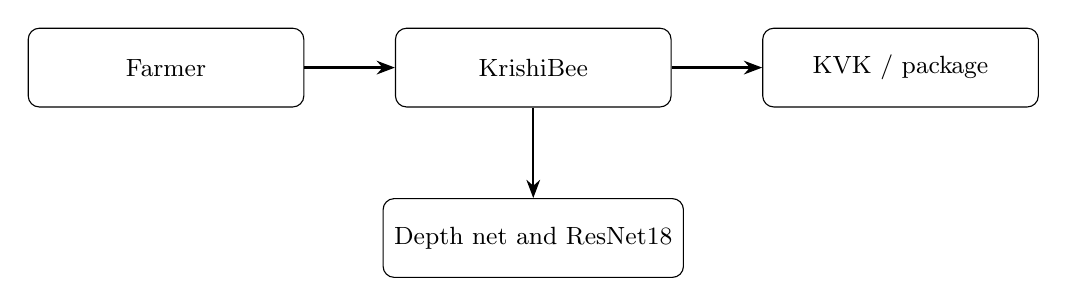
\begin{tikzpicture}[
    node distance=1.15cm and 1.15cm,
    box/.style={draw, rounded corners, align=center, minimum width=3.5cm, minimum height=1cm, font=\small, inner sep=4pt},
    arr/.style={-{Stealth}, thick}
]
    \node[box] (farmer) {Farmer};
    \node[box, right=of farmer] (app) {KrishiBee};
    \node[box, right=of app] (kvk) {KVK / package};
    \node[box, below=of app] (models) {Depth net and ResNet18};
    \draw[arr] (farmer) -- (app);
    \draw[arr] (app) -- (kvk);
    \draw[arr] (app) -- (models);
\end{tikzpicture}
\caption{The farmer sends a field, a date, or a photograph to KrishiBee. The package and the KVK remain the authority for practice. The models supply a depth and a wheat-photo score, each shown with its limit.}
\label{fig:stakeholders}
\end{figure}

\section{Functional Requirements}
Table~\ref{tab:fr} lists the behaviours the deployed system is required to provide. Each one is visible on the live site or on a documented API route.

\begin{table}[H]
\centering
\caption{Functional requirements.}
\label{tab:fr}
\small
\begin{tabularx}{\textwidth}{lX}
\toprule
\textbf{ID} & \textbf{Requirement} \\
\midrule
FR1 & Given a crop, state, season and point inside that state, return the network depth, the rule depth and the safe range. \\
FR2 & If the live soil query fails, say that a cached nearby point was used, and give the distance. \\
FR3 & Reject a point that does not lie inside the selected state. \\
FR4 & Answer a question from at most three matching notes, and list the sources. If none match, say so and direct the user to the KVK. \\
FR5 & Build a crop calendar from a sowing or transplanting date for wheat, chickpea, mustard and rice, including a warning when wheat is outside the timely window. \\
FR6 & On a wheat plan, match a photograph only to identifiers in the PAU problem list, and show the ResNet18 class beside that list. \\
FR7 & Withhold the ResNet18 name when the calibrated probability is below 0.8. \\
FR8 & After a field is chosen, show seven days of rain and temperature and name the next open task on a saved plan. \\
\bottomrule
\end{tabularx}
\end{table}

\section{Non-Functional Requirements}
\begin{itemize}[leftmargin=1.4em]
    \item \textbf{Traceability.} A numerical claim about irrigation, fertiliser or depth range is either in a retrieved note, on a calendar task, or in the rule table. The language model is not a source of new numbers.
    \item \textbf{Privacy.} Plans live in browser storage. Photographs live in IndexedDB, compressed so that the long side is at most 1280 pixels. The photo-check request is not written to a database.
    \item \textbf{Honesty of metrics.} Depth scores are described as agreement with the rule engine. Classifier scores are described as performance on the John Innes Centre subset.
    \item \textbf{Graceful failure.} A paused soil service, a sleeping API, a missing Groq key, and an unreachable forecast each produce a sentence the user can act on, rather than a blank screen.
    \item \textbf{Language.} The chat accepts Hindi, Hinglish and English. The rest of the interface is English.
    \item \textbf{Limits.} Chat allows 10 requests from one address in 10 minutes and 80 in a day. The photo check allows 6 in 10 minutes and 40 in a day. Both counters live in the API process and reset when that process restarts, so the provider's own limit is the real backstop.
\end{itemize}

\section{Tracing a Requirement to the Screen}
A requirement that cannot be pointed at is not yet a requirement of this system. Table~\ref{tab:fr} is therefore read against the running site, not against a diagram alone.

FR1 is the depth card. After a crop, a state, a season and a point inside that state, the card prints three depths: the network, the rule, and the safe range from Table~\ref{tab:bands}. It also prints the texture class and the estimated moisture, because those are the inputs a reader needs in order to recompute the rule by hand. FR2 is the sentence on that same card when SoilGrids does not answer. The sentence names the distance to the cached soil point. In the session recorded in Chapter~\ref{ch:results} that distance was 23.0\,km, and the card said so. FR3 is the rejection of a click that falls outside the bounding box of the selected state. The message asks the user to click inside the state or to change the state dropdown. The box is a rectangle. It is a guard against evaluating Punjab rules on a click in another state, and it is not a village boundary.

FR4 is the chat under the depth card. A question is searched inside the notes for the current crop. At most three notes that score highly enough are given to the language model, and the page lists those notes under the reply. A question with no adequate note ends in a short refusal and a pointer to the KVK, rather than a timetable invented to fill the silence. The standing warning on the panel says that the notes are a small set and that quantities should be confirmed locally. That warning stays even when the answer is a good one, because the prose can still add a clause the note did not contain.

FR5 is My crop. The farmer enters wheat, chickpea, mustard or rice, and a date. For rice the date is the transplanting date, and the screen says so. Wheat irrigation windows change with the sowing month, which is how the package is written: an October sowing and a December sowing are not given the same interval. A wheat date outside the timely window raises a warning rather than being silently accepted. Tasks can be marked done. The plan stays on the device.

FR6 and FR7 share the photo check, and they are available only after the plan is wheat. The other three crops explain that a photograph will not be scored. On wheat, one path may return only identifiers from the 14-entry PAU list, and the sentences under a match are the list's sentences. The other path is ResNet18. Its class name is printed only when the calibrated probability is at least 0.8. A weaker top class is reported as withheld. The two blocks sit on the same result so that a confident PAU match and a withheld network name can be seen together, as they are for the powdery-mildew photograph in Table~\ref{tab:spot}.

FR8 is the forecast under the map, and again at the top of My crop. Seven days of temperature and rain are requested by the browser. The card names the next open task on the saved plan. The extra sentence, which says to check the field before irrigating, appears only when that task is an irrigation, it starts within seven days, and rain is likely. A weed-control window in a rainy week does not trigger it. The depth numbers do not change when the forecast loads.

The non-functional requirements are visible in the same pass. The source line under a chat answer is the traceability requirement. The absence of an account, and the fact that a second phone does not show the plan, is the privacy requirement. The cold start of the free API host, which can take up to a minute after a quiet period, is the graceful-failure requirement in its slow form. A faster failure has a sentence: soil data replaced by a named cache, chat or photo check not configured, the photo service unreachable, or a rate limit asking the user to wait. None of those sentences is a blank panel.


\chapter{System Design}
\label{ch:design}

\section{Overall Architecture}
KrishiBee is a browser client and a small HTTP API. The client holds the map, the forms, the calendar and the photographs. The API holds the depth model, the wheat classifier, the note index and the calls to the language and vision models. The seven-day forecast is the exception: the browser calls Open-Meteo directly, because the free API host could not complete that call reliably.

\begin{figure}[H]
\centering
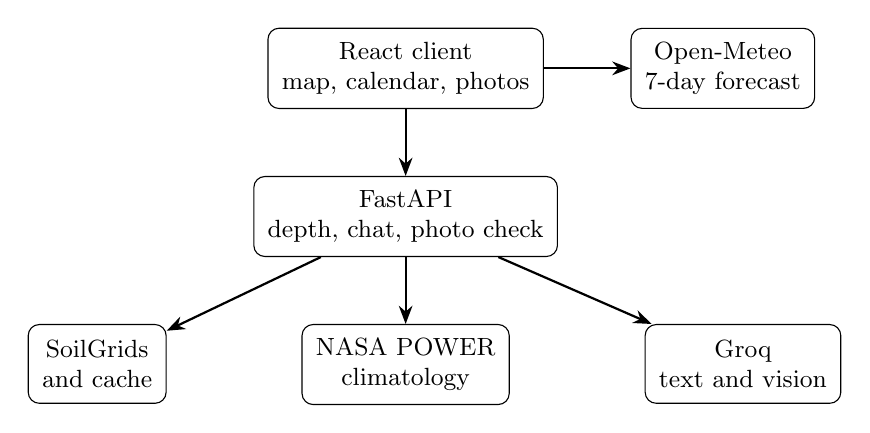
\begin{tikzpicture}[
    node distance=0.85cm and 1.1cm,
    box/.style={draw, rounded corners, align=center, minimum height=1cm, font=\small, inner sep=5pt},
    arr/.style={-{Stealth}, thick}
]
    \node[box] (ui) {React client\\ map, calendar, photos};
    \node[box, right=of ui] (meteo) {Open-Meteo\\ 7-day forecast};
    \node[box, below=of ui] (api) {FastAPI\\ depth, chat, photo check};
    \node[box, below left=of api] (soil) {SoilGrids\\ and cache};
    \node[box, below=of api] (power) {NASA POWER\\ climatology};
    \node[box, below right=of api] (groq) {Groq\\ text and vision};
    \draw[arr] (ui) -- (api);
    \draw[arr] (ui) -- (meteo);
    \draw[arr] (api) -- (soil);
    \draw[arr] (api) -- (power);
    \draw[arr] (api) -- (groq);
\end{tikzpicture}
\caption{The client calls the API for depth, chat and photo check. The week forecast is requested by the browser.}
\label{fig:arch}
\end{figure}

\section{Depth Data and the Rule Engine}
One hundred and forty-five coordinates were sampled across the five states. At each coordinate the soil properties listed in Chapter~\ref{ch:lit} were stored, and a Rabi row and a Kharif row of climatology were stored. Not every crop is grown in both seasons, so the synthesised table has 1{,}160 rows rather than $145 \times 8 \times 2$. Each row is passed through \texttt{crop\_database.py}, which holds a base depth interval and additive adjustments for texture, moisture, expected rain and temperature. A small amount of noise is added so that the labels are not a perfect function of the inputs. The safe range shown in the app is the audited base interval, not the noisy label.

The adjustment for texture is a fixed step: $+0.5$\,cm on sand, $+0.3$\,cm on sandy loam, zero on loam, $-0.3$\,cm on clay loam, and $-0.5$\,cm on clay. The other three adjustments are functions, written here so that a depth on the card can be recomputed without opening the code. Let $m$ be the estimated moisture in percent. The moisture term is
\begin{equation}
\delta_{m} =
\begin{cases}
0.6 & m \le 5, \\[2pt]
0.6 \cdot (20-m)/15 & 5 < m \le 20, \\[2pt]
-0.4 \cdot (m-20)/15 & 20 < m \le 35, \\[2pt]
-0.4 & m > 35.
\end{cases}
\label{eq:moisture}
\end{equation}
It is $+0.6$\,cm on a very dry surface, zero at 20\%, and $-0.4$\,cm once the estimate reaches 35\%. Let $r$ be the seven-day rainfall in millimetres. Rain contributes nothing unless the rain flag is set. When it is set,
\begin{equation}
\delta_{r} = \max\big(-0.55,\; -0.2 - \min(0.35,\; (r-5)\cdot 0.35/25)\big).
\label{eq:rain}
\end{equation}
Once the seven-day rainfall rises above 5\,mm the shallowing gets stronger, and it stops at $-0.55$\,cm. Temperature adds a cold term and a hot term. The cold term is used only in Rabi and only below 18\,$^{\circ}$C:
\begin{equation}
\delta_{\mathrm{cold}} = \max\big(-0.4,\; (T-18)\cdot(-0.4)/(5-18)\big).
\label{eq:cold}
\end{equation}
It is zero at 18\,$^{\circ}$C and reaches $-0.4$\,cm at 5\,$^{\circ}$C. Above 32\,$^{\circ}$C, in either season,
\begin{equation}
\delta_{\mathrm{hot}} = \min\big(0.5,\; (T-32)\cdot 0.5/(45-32)\big),
\label{eq:hot}
\end{equation}
which reaches $+0.5$\,cm at 45\,$^{\circ}$C and does not grow after that. The recommended depth is the optimal depth plus the four terms, clipped to the audited band extended by 0.3\,cm:
\begin{equation}
d = \mathrm{clip}\big(d_{\mathrm{opt}} + \delta_{\mathrm{texture}} + \delta_{m} + \delta_{r} + \delta_{T},\; d_{\min}-0.3,\; d_{\max}+0.3\big).
\label{eq:depth}
\end{equation}
Wheat uses $d_{\mathrm{opt}}=5.0$, $d_{\min}=4$ and $d_{\max}=6$, so the clip allows 3.7\,cm to 6.3\,cm. The number printed as the safe range remains 4--6\,cm. The rule depth is allowed to sit up to 0.3\,cm outside that printed range when the adjustments pile up. Showing both numbers is the point of the card: the range is the package interval, and the rule depth is the interval after soil and weather.

The training label is not $d$ itself. After $d$ is computed, a Gaussian draw with mean zero and standard deviation 0.15\,cm is added and the same clip is applied. The synthesis uses a fixed seed, so the table is reproducible. The noise stops the network from being scored as if it had to copy a deterministic formula to the last hundredth of a centimetre. It also means the irreducible error on this table sits near 0.15\,cm before the clip removes some of the variance. At inference the API evaluates the clean rule, with no new draw of noise, and returns that depth beside the network. A gap between them is expected even when the network has learned the table well.

That arithmetic is why a live card can be checked by hand. On the deployed example in Chapter~\ref{ch:results}, the field was reported as loam with estimated moisture 24.43\%. Texture contributes 0. Equation~\eqref{eq:moisture} at 24.43\% contributes $4.43 \times (-0.4)/15$, which is about $-0.12$\,cm. Starting from 5.0\,cm, the rule lands at 4.88\,cm when rain and temperature contribute nothing further. The network returned 4.95\,cm. Both sit inside 4--6\,cm. The gap of 0.07\,cm is smaller than the 0.15\,cm noise and smaller than the deployed test MAE of 0.151\,cm. It is the sort of disagreement the card is meant to show.

A second numerical example, not taken from the live site, shows the clip working. Take wheat on sand, with estimated moisture 10\%, no rain flag, and a Rabi temperature of 14\,$^{\circ}$C. Texture contributes $+0.5$\,cm. Moisture contributes $+0.4$\,cm. Equation~\eqref{eq:cold} contributes $-0.123$\,cm. The sum is 5.78\,cm, still inside 3.7--6.3\,cm, so the clip does nothing and the rule depth is 5.78\,cm against a printed range of 4--6\,cm. Change the same crop to clay, moisture 40\%, rain expected with 30\,mm in the window, and temperature 22\,$^{\circ}$C. Texture contributes $-0.5$\,cm, moisture $-0.4$\,cm and rain $-0.55$\,cm. The raw sum is 3.55\,cm, and the clip raises it to 3.70\,cm. The card would then show a rule depth of 3.70\,cm beside a safe range of 4--6\,cm. That is a legal output of Equation~\eqref{eq:depth}. It is also a reason not to hide the range behind a single ``recommended'' number.

When SoilGrids does not answer, the API computes the great-circle distance to every cached soil point and uses the nearest one. The response states the distance in kilometres. A point outside the bounding box of the selected state is rejected before any lookup. That check is deliberately simple. It stops a Punjab query from being evaluated on a click in another state. It is not a cadastral boundary.

\section{AgroDynamicNet}
AgroDynamicNet has three branches, each ending in a 32-unit representation. The soil branch reads eleven features: sand, clay, silt, pH, nitrogen, organic carbon, bulk density, estimated moisture, estimated phosphorus, estimated potassium, and an encoded texture class. The weather branch reads temperature, humidity, seven-day rainfall, solar radiation, wind, a rain flag, a season code and the sowing month. The crop branch embeds the crop name in eight dimensions and the state in four, then concatenates seed size, thousand-seed weight, latitude and longitude. Dropout on the branches is 0.15, with batch normalisation. The three vectors are concatenated into a trunk of width 64, then 32, then a single depth output. Figure~\ref{fig:net} shows the merge.

\begin{figure}[H]
\centering
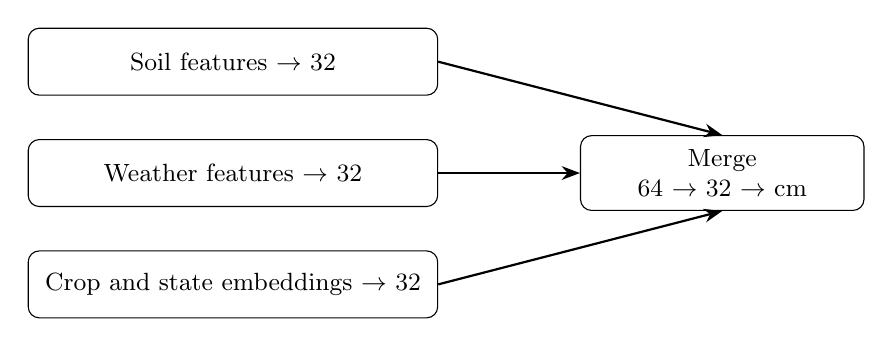
\begin{tikzpicture}[
    node distance=0.55cm and 1.8cm,
    box/.style={draw, rounded corners, align=center, font=\small, minimum width=5.2cm, minimum height=0.85cm, inner sep=4pt},
    mergebox/.style={draw, rounded corners, align=center, font=\small, minimum width=3.6cm, minimum height=0.95cm},
    arr/.style={-{Stealth}, thick}
]
    \node[box] (s) {Soil features $\rightarrow$ 32};
    \node[box, below=of s] (w) {Weather features $\rightarrow$ 32};
    \node[box, below=of w] (c) {Crop and state embeddings $\rightarrow$ 32};
    \node[mergebox, right=of w] (m) {Merge\\ 64 $\rightarrow$ 32 $\rightarrow$ cm};
    \draw[arr] (s.east) -- (m.north);
    \draw[arr] (w.east) -- (m.west);
    \draw[arr] (c.east) -- (m.south);
\end{tikzpicture}
\caption{AgroDynamicNet. Any branch can be replaced by zeros for the ablation. There is no recurrent layer, because the weather input is one climatology vector per season.}
\label{fig:net}
\end{figure}

The forward pass takes three flags, \texttt{use\_soil}, \texttt{use\_weather} and \texttt{use\_crop}. Setting a flag to false replaces that branch with zeros. The ablation is therefore the same code path as the deployed model, not a separately designed network. The weights loaded by the API are from one training run. The five-seed study was run without replacing those weights.

The loss is mean squared error on the noisy depth in centimetres. Training uses Adam with learning rate $10^{-3}$, weight decay $10^{-5}$ and batches of 32. A run may last 300 epochs. It stops earlier when the validation MAE has not improved for 25 epochs, and the weights that are kept are the ones with the best validation MAE, not the weights of the final epoch. The same loop fits the combined network and the three ablations. Only the flags change. Because the deployed file is an earlier run, its test MAE of 0.151\,cm is reported separately from the five-seed mean. It happens to sit inside the range of those seeds. It is not defined to be one of them.

\section{Retrieval and the Chatbot}
Notes live in JSON, one file per crop. A note has an identifier, a crop, a topic string, a short paraphrase, a source title and a source URL where one exists. At startup the API builds a BM25 index and a small map from Hindi and Hinglish words onto the English terms used in the notes. A query is expanded, then searched inside the current crop. The top three notes, if any score highly enough, are placed in the prompt with the latest depth context: crop, state, season, recommended depth, safe range, texture and estimated moisture.

The system instruction tells the model to use a number only when it appears in those notes, to avoid pesticide and fertiliser doses from memory, and to send the farmer to the KVK when the notes are silent. The API returns the sources separately, so the page can render them even if the prose forgets to. Weak matches are dropped rather than passed in as if they were evidence. Crops with no file produce an up-front notice instead of a pretended answer.

\section{Crop Calendar}
The calendar is a table, not a model. For each of wheat, chickpea, mustard and rice, the file \path{schedules.json} stores tasks with a start and end counted from the entered date, or a calendar date such as the opening of yellow-rust scouting. Wheat irrigation has variants: the interval depends on whether sowing was in October, early November, late November or December. A task can share the window of another task, which is how the urea applications stay tied to the irrigations. Rice uses the entered date as transplanting, and the direct-seeded timings are written in the task note.

A task is due when today falls inside its window, upcoming before that, and passed after the window plus a grace period. The farmer can mark a task done. The plan is stored under one browser key. Removing the plan clears the photographs as well.

\section{Photo Check}
The wheat problem list contains 14 entries: eight diseases, two pests and four nutrient deficiencies, each with what to look for, what the package says, and the page. The vision model receives the photograph and the list of identifiers. Any identifier it returns that is not on the list is discarded. The sentences shown for a match are copied from the list, not from the model. If the photograph is unreadable, is not wheat, or matches nothing, the page says so. Ranks are shown without a confidence percentage, because that model does not produce a calibrated one.

The ResNet18 path is independent. The image is decoded, resized to $224 \times 224$, and normalised as for ImageNet. Logits are divided by a temperature of $0.8484$ fit on the validation split of seed 0, then turned into a probability. The class is reported only when the top probability is at least 0.8. Otherwise the page says the network is not confident enough to name a class. The note under the score states the training geography and the five class names. MobileNetV3-Small was trained in the same harness and is not loaded by the API.

\begin{figure}[H]
\centering
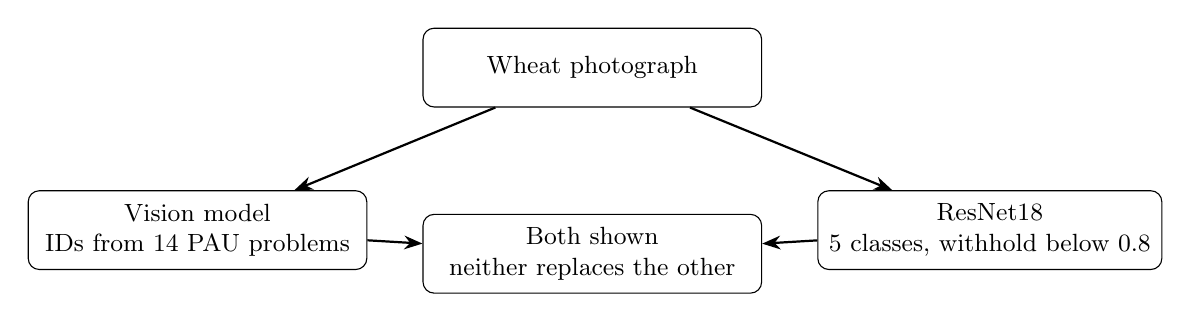
\begin{tikzpicture}[
    node distance=1.05cm and 0.7cm,
    box/.style={draw, rounded corners, align=center, font=\small, minimum width=4.3cm, minimum height=1cm, inner sep=4pt},
    arr/.style={-{Stealth}, thick}
]
    \node[box] (photo) {Wheat photograph};
    \node[box, below left=of photo] (groq) {Vision model\\ IDs from 14 PAU problems};
    \node[box, below right=of photo] (net) {ResNet18\\ 5 classes, withhold below 0.8};
    \node[box, below=1.35cm of photo] (out) {Both shown\\ neither replaces the other};
    \draw[arr] (photo) -- (groq);
    \draw[arr] (photo) -- (net);
    \draw[arr] (groq) -- (out);
    \draw[arr] (net) -- (out);
\end{tikzpicture}
\caption{The photo check has two outputs. The PAU list is the practice advice. The ResNet18 score is a calibrated class from a different dataset.}
\label{fig:photopath}
\end{figure}

\section{Week Forecast}
The forecast card requests seven daily values from Open-Meteo: weather code, maximum and minimum temperature, precipitation sum, and precipitation probability \cite{openmeteo}. A day is treated as likely rain when the sum is at least 1\,mm or the probability is at least 50\%. The card then reads the crop plan saved on the device, skips tasks that are marked done or whose window has passed, and names the next remaining task. The stronger sentence, which tells the farmer to check the field before irrigating, is used only when that task is an irrigation, it starts within seven days, and rain is likely. The card never says to skip the irrigation.

An API route for the same forecast exists and works from a developer machine. It is not what the live site calls. The hosted process received an error from Open-Meteo and turned that into an HTTP 502. Moving the request into the browser removed that dependency. The depth model is unchanged.

\section{Deployment}
The client is a Vite build hosted on Vercel. The API is FastAPI on Render, started with one worker. Cross-origin access is limited to an environment list. The Groq key is an environment variable and is not in the repository. Model weights for AgroDynamicNet and for the seed-0 ResNet18 are loaded at process start. The first user request after sleep pays the cold-start cost of that host.


\chapter{Implementation}
\label{ch:impl}

\section{Development Environment}
Training was done in Python with PyTorch, scikit-learn and XGBoost. The API dependency file is shorter: FastAPI, Uvicorn, a CPU build of PyTorch and TorchVision, pandas, requests and Pydantic. The client is React, bundled with Vite, with Leaflet for the map and Axios for the API. Photographs are stored with the browser's IndexedDB. Versions are pinned for the torch packages in the deploy file so the hosted build does not drift.

Locally, the API is started with \path{uvicorn api.main:app --reload --port 8000} after the Groq key is set in the shell. The client reads \path{VITE_API_BASE} and otherwise uses \path{http://localhost:8000}. A separate flag turns off the in-memory photo-check cap for a local evaluation only. It is not set on the host.

\section{Data and Training Programs}
\texttt{scripts/collect\_soil\_data.py} and \texttt{scripts/collect\_weather\_data.py} write the raw point tables. \texttt{scripts/synthesize\_dataset.py} joins them to crops and applies the rule engine. \texttt{scripts/validate\_dataset.py} checks the joined table. \texttt{scripts/prepare\_final\_dataset.py} writes the train, validation and test splits and the scaler. \texttt{scripts/train\_baseline\_models.py} fits Random Forest and XGBoost. \texttt{scripts/train\_nn.py} fits AgroDynamicNet, including the branch ablations. Repeated seeds write a report per seed and do not overwrite the weights the API loads.

\texttt{scripts/train\_wheat\_classifier.py} fine-tunes either ResNet18 or MobileNetV3-Small. The 40 pilot files are excluded by hash. The remaining images are split once, with a fixed split seed, into 671 training, 144 validation and 144 test images, and that split is reused for every model seed. The script records accuracy, macro-F1, a temperature, an expected calibration error before and after scaling, and a coverage table at several probability thresholds. \texttt{scripts/gradcam\_wheat.py} can draw a Grad-CAM map for the ResNet18 checkpoint \cite{selvaraju2017gradcam}. That script is an analysis tool. The website does not call it.

\texttt{scripts/sample\_eval.py} draws the 40-image pilot, ten images each of yellow rust, brown rust, powdery mildew and healthy leaves. Septoria is one of the five training classes and is not in the pilot folders. \texttt{scripts/eval\_diagnose.py} sends the pilot through the photo-check endpoint once, without any change to the prompt in response to the scores.

\section{How the Two Models Are Fit}
The depth labels are built before any network is trained. Soil and weather are joined on location and season. Each crop is attached only to its season. The rule of Chapter~\ref{ch:design} produces a depth, noise of standard deviation 0.15\,cm is added, and the row is clipped. The training script then standardises the numeric inputs with means and standard deviations stored beside the split, so the API can apply the same scale at inference. Crop name and state are integer codes into the two embedding tables. A branch that the ablation turns off is replaced by a zero vector of width 32 after that branch would have run, which keeps the trunk the same shape for every variant.

The wheat classifier starts from an ImageNet checkpoint. Training images are randomly cropped to $224 \times 224$ with a scale down to half the frame, flipped on either axis, rotated by up to 20 degrees, and jittered in brightness, contrast, saturation and hue. Validation, test and pilot images are only resized to $224 \times 224$ and normalised with the ImageNet mean and standard deviation. The 40 pilot files are removed by an MD5 hash of the file bytes before the split, so a renamed copy does not leak back into training. The remaining images are split once, stratified by class, with split seed 42: 70\% train and 30\% held out, and that held-out half is split again into validation and test. The counts are 671, 144 and 144. Every model seed reuses the split. What changes with the seed is the initialisation noise, the order of the training batches, and the dropout masks.

The classifier loss is cross-entropy with class weights inverse to the training counts, and with label smoothing of 0.05. The optimiser is AdamW. The pretrained backbone uses learning rate $10^{-4}$ and the new classification head uses $10^{-3}$, with weight decay $10^{-4}$. A cosine schedule runs over a maximum of 20 epochs. The checkpoint that is restored is the one with the best validation macro-F1, and training stops after six epochs without an improvement. Temperature scaling is fit afterwards, on the validation logits of that checkpoint, by minimising cross-entropy over a single positive temperature with LBFGS. The temperature does not change which class wins. It changes the probability that is compared with 0.8. Expected calibration error on the test split uses ten equal-width bins of that probability. The API loads the seed-0 ResNet18 weights and the temperature stored with them, 0.8484. MobileNetV3-Small is trained in the same harness so that the five-seed table has a smaller baseline. Its weights are not loaded.

Random Forest and XGBoost are fit on the same depth split as comparators. The forest has 300 trees with a maximum depth of 12. The boosted model has 300 trees, a maximum depth of 6 and a learning rate of 0.05. Both use a fixed random seed. A five-fold cross-validation MAE is computed on the training rows only, as a check that the test number is not a single lucky partition. Those models are not served. Serving them would have given up the branch flags, which are the reason the ablation and the deployed network are the same architecture.

\section{API Modules}
\path{api/main.py} loads AgroDynamicNet. It exposes \path{/health}, \path{/crops}, \path{/predict} and \path{/predict_by_location}, and includes the other routers. \texttt{/predict} accepts soil and weather fields directly, which is how a developer can bypass the live lookups. \texttt{/predict\_by\_location} is what the page uses.

\texttt{api/retrieval.py} tokenises notes, expands the Hindi and Hinglish map, and ranks with BM25. \texttt{api/chat.py} applies the rate limit, builds the prompt and returns the answer with the notes that were used. \texttt{api/diagnose.py} loads the problem list, calls the vision model, filters identifiers, and, when the crop is wheat, calls \texttt{api/wheat\_classifier.py}. That module decodes the image, applies the ImageNet transform, scales the logits by the stored temperature, and sets \texttt{abstained} when the top probability is below 0.8. \texttt{api/forecast.py} is the server-side forecast used in local tests. The page no longer calls it.

\section{Client Modules}
The depth screen is a map and a form. Choosing a point stores the latitude and longitude in the browser so that My crop can show the same forecast. The result card prints the network depth, the rule depth, the safe range, the texture, the estimated moisture, and a note when cached soil was used. The chat panel sits under that card and sends the latest result as context. Suggested questions are starting points only.

My crop is a second view, not a second site. Before a plan exists it asks for the crop and the date. After that it lists tasks in date order with a status chip and a checkbox. The forecast card is the first block on that view as well. The photo timeline accepts a camera capture or a file, compresses it, and shows the check button only for wheat. The result component renders the PAU matches and, when present, the ResNet18 block with its probability or its withheld message.

The advisor layout places the map and the forecast in the left column and the form, the depth card and the chat in the right column. On a narrow screen the same blocks stack in that order. This is a presentation change. It does not change a prediction.

\section{One Depth Request, End to End}
A click on the map stores the latitude and longitude in the page and in browser storage. The form sends the crop, the state, the season and that point to \path{/predict_by_location}. The API checks that the season is known and that the point lies inside the bounding box of the selected state. It then asks SoilGrids for sand, clay, pH, organic carbon, bulk density and nitrogen, with a short timeout and a single retry. If any of those fields is missing, it replaces the soil record with the nearest cached point and keeps the distance.

Climatology for the same point is read next. The season's row supplies temperature, humidity, rainfall, the rain flag, solar radiation, wind and the sowing month. Phosphorus, potassium and moisture are estimated from the soil record by the same functions used in training. Those values, together with the crop's seed size and seed weight, are scaled with the stored training means and standard deviations and passed through AgroDynamicNet. The rule engine is called on the unscaled values. The response contains both depths, the safe range, the texture class, the moisture estimate, and a note. The note is where a cached-soil distance is written. The page does not choose between the two depths. It prints them side by side.

A photo check is a different request. The browser resizes the image and sends it, with the crop name, to \path{/diagnose}. For wheat, the server runs the vision-model match against the 14 identifiers and, separately, \path{classify_base64} on the ResNet18. The JSON that comes back has the PAU candidates and a classifier object with the label, the probability, the threshold, and whether the call was withheld. The page renders those fields. It does not recompute the threshold.

\section{What the Page Does When a Service Fails}
The free hosts fail in ways a demonstration has to absorb. SoilGrids is queried with a short timeout and one retry. If sand, clay, pH, organic carbon, bulk density or nitrogen is missing, the API replaces the soil record with the nearest cached point and writes the distance into the note. If the cache itself is empty, the request fails with a sentence that says live soil data is unavailable. Weather for the depth model is the stored climatology for that point and season. If that lookup fails, the page says the weather could not be fetched, and it does not invent a climate in the browser.

A point outside the rectangle of the selected state is rejected before either lookup. The message names the state and asks for a click inside it, or for the dropdown to be changed. Chat without a key on the server says that chat is not configured. A photo check without a key says the same about the photo check. If the language or vision service is unreachable, or returns nothing usable, the page says so and asks for another try. It does not fill the gap with a depth-only answer pretending to be a diagnosis.

The photo-check counter allows 6 requests from one address in a window of 600 seconds, and 40 in a day. Chat allows 10 in the same window and 80 in a day. Both counters are in the process memory. Restarting the API clears them, which is useful on a developer machine and is also why the provider's own quota is the limit that matters on the host. A local evaluation of the 40-image pilot sets a flag that disables the photo-check counter. That flag is not set in the deployed environment.

The forecast route on the API is still present and returns a clear failure when the host cannot reach Open-Meteo. The live page does not call that route. The browser calls Open-Meteo itself, which succeeds from the networks on which the host's outbound call did not. If the browser call fails, the card says the forecast is unavailable and leaves the depth card as it was. The next-task line is computed from the plan in local storage, so it can still name a task when the weather request fails, and it stays silent when no plan has been saved.

\section{What Is Stored Where}
Table~\ref{tab:storage} is the privacy boundary of the system. It is also the reason a plan does not follow the farmer to a second phone.

\begin{table}[H]
\centering
\caption{Where each piece of farmer data lives.}
\label{tab:storage}
\small
\begin{tabularx}{\textwidth}{lX}
\toprule
\textbf{Data} & \textbf{Where it is kept} \\
\midrule
Soil cache and model weights & On the API host, built before deployment \\
Chat and photo-check requests & Sent for an answer, not written to an application database \\
Crop plan & \texttt{localStorage} on the device \\
Field photographs & IndexedDB on the device, long side at most 1280\,px \\
Last map point & \texttt{localStorage}, so the forecast can reload \\
Groq credential & Host environment variable, not in the repository \\
\bottomrule
\end{tabularx}
\end{table}

\section{Repository Layout}
\texttt{scripts/} holds collection, synthesis, training and evaluation. \texttt{models/} holds the AgroDynamicNet definition and the two weight files the API loads. \texttt{api/} holds the HTTP layer. \texttt{frontend/} holds the client, including \texttt{src/data/schedules.json}. \texttt{data/knowledge/} holds the paraphrased notes. \texttt{data/problems/} holds the wheat problem list. \texttt{data/processed/} holds the metric reports for every seed. The wheat photographs themselves are not in the repository.


\chapter{Results}
\label{ch:results}

\section{How the Depth Numbers Should Be Read}
Every depth label is the output of the rule engine, plus a little noise. A low error means the model has learned those rules. It does not mean a field trial measured emergence. The test set is a held-out portion of the same synthetic table. Random Forest importance puts crop identity at about 87\% of the split, which is expected: chickpea sits near 11\,cm and mustard near 4.5\,cm, so knowing the crop already explains most of the variance. Within a crop, Random Forest $R^{2}$ still runs from 0.72 for mustard to 0.95 for maize, so the remaining features are not empty. They are smaller than the crop effect.

\section{Single Split Served by the Application}
Table~\ref{tab:depth-one} is the run whose neural-network weights the website loads. The tree models were fit on the same split and are not served.

\begin{table}[H]
\centering
\caption{Test error on the single split used for the deployed depth network. Lower MAE is closer agreement with the rule labels.}
\label{tab:depth-one}
\begin{tabular}{lrr}
\toprule
\textbf{Model} & \textbf{Test MAE (cm)} & \textbf{Test $R^{2}$} \\
\midrule
Random Forest & 0.131 & 0.996 \\
XGBoost & 0.133 & 0.996 \\
AgroDynamicNet, all branches & 0.151 & 0.994 \\
AgroDynamicNet, crop only & 0.261 & 0.985 \\
AgroDynamicNet, soil only & 1.500 & 0.194 \\
AgroDynamicNet, weather only & 1.416 & 0.376 \\
\bottomrule
\end{tabular}
\end{table}

The trees are ahead of the network by about two tenths of a millimetre on this split. That gap is smaller than the 0.15\,cm noise added when the labels were built, so it is not a reason to prefer a tree in the product. The network is the model that can zero out a branch, which is why it is the one discussed in the ablation and the one loaded by the API. Soil alone and weather alone do not predict depth. Crop identity does. The useful question is the gap between crop-only and the full network.

Two further checks keep the single-split table from being read as a lucky test. On the training rows, five-fold cross-validation MAE is 0.141\,cm for the forest and 0.142\,cm for the boosted trees, each with a fold-to-fold standard deviation below 0.01\,cm. Those training figures sit close to the test figures in Table~\ref{tab:depth-one}. Inside the forest, the encoded crop name accounts for 0.874 of the impurity reduction. The next features are the seven-day rainfall, seed size and thousand-seed weight, each below 0.04. The boosted model also puts the crop first, and then the sowing month, which is tied to season. Within one crop the forest still has something to fit: $R^{2}$ runs from 0.72 on mustard to 0.95 on maize, with wheat at 0.80. The remaining features are real. They are much smaller than the jump from mustard at 4.5\,cm to chickpea at 11.25\,cm.

\section{Five Seeds and the Branch Ablation}
Five additional seeds were trained without replacing the deployed weights. Table~\ref{tab:depth-seeds} summarises them.

\begin{table}[H]
\centering
\caption{Five-seed depth results. The deployed weights are the earlier single run in Table~\ref{tab:depth-one}, whose MAE of 0.151\,cm sits inside the combined-network range below.}
\label{tab:depth-seeds}
\begin{tabular}{lrr}
\toprule
\textbf{Variant} & \textbf{Test MAE (cm)} & \textbf{Test $R^{2}$} \\
\midrule
Combined & $0.166 \pm 0.018$ & $0.994 \pm 0.001$ \\
Crop only & $0.256 \pm 0.009$ & $0.986 \pm 0.001$ \\
Soil only & $1.531 \pm 0.026$ & $0.171 \pm 0.028$ \\
Weather only & $1.418 \pm 0.025$ & $0.397 \pm 0.023$ \\
\bottomrule
\end{tabular}
\end{table}

Relative to the crop-only network, the combined network reduces MAE by 35.2\% on average. The arithmetic of that sentence is $(0.256 - 0.166) / 0.256$. The five seeds do not share the reduction equally. Table~\ref{tab:depth-by-seed} gives the test MAE of the combined network and of the crop-only network on each seed. The reduction is $(m_{\mathrm{crop}} - m_{\mathrm{full}}) / m_{\mathrm{crop}}$.

\begin{table}[H]
\centering
\caption{Test MAE in centimetres on each depth seed, to four decimal places. The reduction is computed from the unrounded errors and can differ in the second decimal from a ratio of the printed values. These runs did not replace the weights loaded by the API.}
\label{tab:depth-by-seed}
\begin{tabular}{rrrr}
\toprule
\textbf{Seed} & \textbf{Combined} & \textbf{Crop only} & \textbf{Reduction} \\
\midrule
0 & 0.1618 & 0.2477 & 34.7\% \\
1 & 0.1579 & 0.2549 & 38.0\% \\
2 & 0.1503 & 0.2673 & 43.8\% \\
3 & 0.1631 & 0.2469 & 33.9\% \\
4 & 0.1965 & 0.2632 & 25.3\% \\
\bottomrule
\end{tabular}
\end{table}

\begin{figure}[H]
\centering
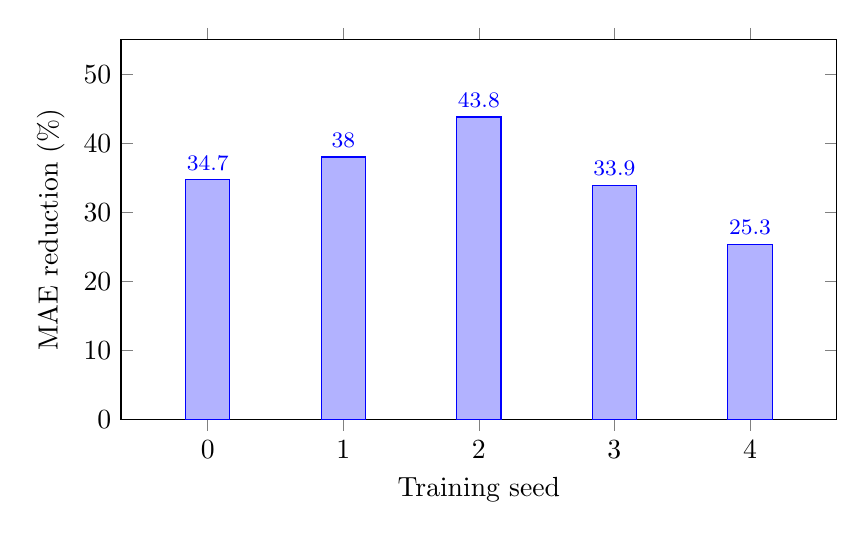
\begin{tikzpicture}
\begin{axis}[
    ybar,
    bar width=16pt,
    width=0.88\textwidth,
    height=6.4cm,
    ylabel={MAE reduction (\%)},
    xlabel={Training seed},
    symbolic x coords={0,1,2,3,4},
    xtick=data,
    ymin=0,
    ymax=55,
    nodes near coords,
    every node near coord/.append style={font=\footnotesize, /pgf/number format/fixed, /pgf/number format/precision=1},
    enlarge x limits=0.16,
    ytick={0,10,20,30,40,50},
]
\addplot coordinates {(0,34.7) (1,38.0) (2,43.8) (3,33.9) (4,25.3)};
\end{axis}
\end{tikzpicture}
\caption{Seed-wise reduction in test MAE when soil and weather are added to the crop-only network. The mean is 35.2\% and the sample standard deviation is 6.7 percentage points. Seed 4 is the low value.}
\label{fig:reduction}
\end{figure}

Four of the five seeds land between 0.1503 and 0.1631\,cm. Seed 4 lands at 0.1965\,cm, which is why the combined standard deviation is 0.018\,cm rather than a much smaller number. That seed is still 0.067\,cm closer to the labels than its own crop-only run, and it remains far below the soil-only and weather-only errors near 1.5\,cm. The study does not contain a seed in which adding soil and weather made the error worse. It does contain a seed whose gain is about 25\% rather than about 40\%, so the mean of 35.2\% should be quoted with the 6.7 point spread beside it. Soil alone ($R^{2}$ about 0.17) and weather alone ($R^{2}$ about 0.40) confirm that the gain is a joint effect. Neither branch is a hidden copy of the crop name.

Before the PAU range audit, on the same split, Random Forest was at 0.127\,cm / 0.989, XGBoost at 0.121\,cm / 0.990, the combined network at 0.153\,cm / 0.985 and the crop-only network at 0.208\,cm / 0.972. $R^{2}$ rose after the audit mostly because the crops moved further apart in depth. Those earlier reports are kept in the repository and are not the numbers the app should be quoted on.

\section{Vision-Model Pilot}
Forty photographs were drawn at random with a fixed seed: ten yellow rust, ten brown rust, ten powdery mildew and ten healthy. They were sent through the photo-check endpoint once. Nothing in the prompt was edited afterwards. Table~\ref{tab:pilot} records that pass. The interval is a 95\% interval on a sample of 30 diseased images, and it is wide.

\begin{table}[H]
\centering
\caption{Pilot of the PAU-list photo check on 40 John Innes Centre images. This pass does not use the ResNet18 score.}
\label{tab:pilot}
\begin{tabular}{lr}
\toprule
\textbf{Outcome} & \textbf{Count} \\
\midrule
Diseased images, correct first answer & 20 of 30 (67\%, interval 49--81\%) \\
Diseased images, correct disease in the top three & 21 of 30 (70\%, interval 52--83\%) \\
Diseased images with no match returned & 5 of 30 \\
Healthy images with no false alarm & 9 of 10 \\
\bottomrule
\end{tabular}
\end{table}

By class, the first answer was right for brown rust on 7 of 10, powdery mildew on 6 of 10, and yellow rust on 7 of 10. With ten images per class the intervals overlap, so the pilot does not show that one disease is easier. Five diseased images produced an empty list, which is a failure to help and also a refusal to invent a match.

\section{Fine-Tuned Classifiers}
ResNet18 and MobileNetV3-Small were fine-tuned on the other 959 images. The pilot files were excluded by hash before the split, so they are not in the 671 / 144 / 144 counts. Every seed reused that split. Table~\ref{tab:clf} is the five-seed summary.

\begin{table}[H]
\centering
\caption{Five-seed classifier results. Pilot columns count the 30 diseased and 10 healthy held-out photographs. Macro-F1 is on the 144-image test split.}
\label{tab:clf}
\small
\begin{tabular}{lrrrr}
\toprule
\textbf{Model} & \textbf{Accuracy} & \textbf{Macro-F1} & \textbf{Pilot, first} & \textbf{Pilot, healthy} \\
\midrule
ResNet18 & $89.4\% \pm 2.2\%$ & $0.880 \pm 0.023$ & $25.2 \pm 1.3$ of 30 & 9 of 10 \\
MobileNetV3-Small & $75.3\% \pm 1.9\%$ & $0.735 \pm 0.015$ & $24.4 \pm 1.8$ of 30 & $8.8 \pm 0.4$ of 10 \\
\bottomrule
\end{tabular}
\end{table}

On this pilot the vision model's 20 of 30 sits below both means. The comparison favours the classifiers: they trained on the same dataset the pilot photographs come from, and the vision model did not. Thirty diseased photographs are enough to make the gap suggestive and not enough to make it precise. CerealConv's 97.05\% \cite{long2023wheat} is a result on a different protocol and a larger training set. It is not a number KrishiBee missed.

The five ResNet18 seeds are not interchangeable in detail, which is why the mean is reported with a standard deviation. Test accuracy runs from 0.875 on seeds 2 and 4 to 0.924 on seed 3. Macro-F1 runs from 0.857 to 0.915. On the 30 diseased pilot images the seeds score 27, 24, 24, 25 and 26, so the mean of 25.2 has a standard deviation of 1.3 images. Healthy images are 9 of 10 on every seed. MobileNetV3-Small stays near 75\% accuracy and near 0.735 macro-F1, and its healthy count is the only one that moves, at $8.8 \pm 0.4$ of 10. The smaller network is a useful baseline and a poor candidate for the page. The page loads seed 0 of ResNet18, whose accuracy of 0.8889 and macro-F1 of 0.8785 sit inside the five-seed band and slightly below the mean. Choosing the seed with the highest test accuracy after looking at the test split would have inflated the number the farmer sees. That was not done.

The validation temperature of that checkpoint is 0.8484. A temperature below 1 sharpens the distribution: probabilities move away from 0.5, so a class that was already ahead becomes more confident. Expected calibration error, computed in ten equal-width bins, moves from 0.0831 to 0.0712. The change is modest. The operating point does more work than the scaling. At a threshold of 0.5 the seed-0 test keeps 95.1\% of images and is right on 91.2\% of those it keeps. At 0.7 the coverage is 81.9\% and the accuracy is 94.9\%. At 0.8 the coverage is 68.1\% and the accuracy is 95.9\%. At 0.9 the coverage falls to 54.2\% and the accuracy is 94.9\%, a little below the accuracy at 0.8. On 144 images that reversal is a small-sample fact, recorded in Table~\ref{tab:coverage}, and it is not a claim that a stricter threshold is worse in general. The threshold shown to the farmer is 0.8. It names about two thirds of the test images, and the names it keeps are right about 96\% of the time on this split. The coarser summary ``about 70\% coverage and about 95\% accuracy'' is this table, read loosely.

\section{Four Photographs on the Deployed Classifier}
The 40-image pilot has no septoria folder. Septoria remains one of the five classes in the 144-image test split. As a separate check of the deployed card, one image from each pilot folder was sent through the running photo check. Table~\ref{tab:spot} is that check. It is an illustration of the threshold, not a second test set.

\begin{table}[H]
\centering
\caption{One photograph from each pilot class, scored by the deployed ResNet18. A probability below 0.8 is withheld even when the top class is the folder name.}
\label{tab:spot}
\begin{tabular}{llcc}
\toprule
\textbf{File} & \textbf{Top class} & \textbf{Probability} & \textbf{Shown} \\
\midrule
\texttt{brown-rust\_00} & Brown rust & 0.964 & Named \\
\texttt{yellow-rust\_00} & Yellow rust & 0.851 & Named \\
\texttt{healthy\_00} & Healthy & 0.996 & Named \\
\texttt{powdery-mildew\_00} & Powdery mildew & 0.606 & Withheld \\
\bottomrule
\end{tabular}
\end{table}

The powdery-mildew case is the important row. The top class matches the folder and the page still refuses to name it. On that same photograph the PAU-list path described white floury spots and matched powdery mildew. The two paths are allowed to disagree in confidence. The farmer sees both.

\screenshot{figures/photo-named.png}{Photo check on a brown-rust pilot image. The ResNet18 name is shown because the probability is above 0.8.}{fig:photo-named}

\screenshot{figures/photo-withheld.png}{Photo check on the powdery-mildew pilot image. The top class is correct and the probability is 0.606, so the name is withheld.}{fig:photo-withheld}

\section{One Session on the Deployed Site}
The tables above are the evaluation. This section is one pass through the public site, made so that those tables can be pointed at on a screen. The field was a point in Punjab, the crop was wheat, and the season was Rabi. SoilGrids did not answer. The card said that cached soil from 23.0\,km away had been used. The derived texture was loam and the estimated moisture was 24.43\%. The network depth was 4.95\,cm. The rule depth was 4.88\,cm. The safe range printed beside them was 4--6\,cm.

The rule figure is the arithmetic of Chapter~\ref{ch:design}. Wheat starts at an optimal depth of 5.0\,cm. Loam adds nothing. Moisture near 24\% adds about $-0.12$\,cm. The result rounds to 4.88\,cm when the rain and temperature terms are zero. The network is 0.07\,cm away. That is inside the 0.151\,cm test MAE of the deployed weights, and it is not a germination measurement. The cached soil is a real degradation: the texture and moisture are from a point 23\,km away, and the card says so.

The forecast on the same date, 28 October 2026, named rain as likely on 30 October and named the next open task as the weed-control window, then running from 20 October to 4 November. That task is not an irrigation, so the card did not add the ``check the field before you irrigate'' sentence. A later week, or a different sowing date, would. The forecast is not scored in Table~\ref{tab:depth-one} and is not an input to the network.

The chat was asked when to give the first irrigation. The reply placed a light first irrigation after the crop had started to grow, at about three weeks for an early-October sowing and about four weeks for a sowing from mid-October to early November, and it referred to the Punjab loam and the estimated moisture. That is the timetable the ungrounded bot had missed. The page still carries the standing warning that answers are drawn from a small set of notes and that quantities should be confirmed with the KVK. The prose can add a clause that is not in the note. The source line under the answer is what the farmer, and an examiner, should read.

\section{Screens of the Deployed Advisor}
The following figures record the requirements in Table~\ref{tab:fr} on the running site at \url{https://krishi-bee.vercel.app}.

\screenshot{figures/depth.png}{Depth advisor for wheat in Punjab. The card shows the network depth, the rule depth and the 4--6\,cm range together.}{fig:depth}

\screenshot{figures/forecast.png}{Seven-day forecast under the map, including the line that names the next open task.}{fig:forecast}

\screenshot{figures/chat.png}{A sourced answer on first irrigation, with the PAU note listed under the reply.}{fig:chat}

\screenshot{figures/tracker.png}{Wheat calendar after a sowing date, with task windows counted from that date.}{fig:tracker}

\section{Discussion}
The depth result that should be quoted is not the $R^{2}$ of 0.994. Crop identity makes a high $R^{2}$ easy once chickpea and mustard sit far apart. The result that should be quoted is the 0.09\,cm gap between the crop-only MAE and the combined MAE, repeated over five seeds, together with the statement that the labels are rules. The trees winning by a fraction of a millimetre does not change the product decision. The network is what makes the ablation the same model as the deployment.

The classifier result that should be quoted is the pair of coverage and accuracy at 0.8, plus the pilot comparison, plus the geography. A system that names every image at 89\% accuracy would be a worse fit for this interface than a system that names about two thirds of them and is right about 96\% of the time on the test split. The withheld powdery-mildew photograph is the demonstration of that choice.

The forecast has no accuracy table. It is a pass-through of a public forecast, joined to a task the calendar already knew. Its failure mode on the hosted API, and the move into the browser, belong in the report because they change which component the farmer is actually calling.

What the project does not show is a germination count, a Punjab leaf, or a second season of use. Those are the limits in the next chapter, and they are already the limits of the evidence above.


\chapter{Conclusion}
\label{ch:conclusion}

\section{Summary of Findings}
KrishiBee shows a sowing depth that moves with soil and weather, and it shows the rule that the depth was trained to copy. On rule-generated labels the deployed network has a test MAE of 0.151\,cm. Across five seeds the full network is about 35\% closer to those labels than a crop-only network. Soil alone and weather alone explain little. Random Forest and XGBoost are slightly closer still on the served split. None of these figures is a measured germination rate.

The wheat photograph is handled by two mechanisms that are not allowed to impersonate each other. A vision model may only name problems from a 14-entry PAU list, and on a 40-image pilot it placed the correct disease first for 20 of 30 diseased images. A ResNet18 trained on the other 959 images from the same public set reaches $89.4\% \pm 2.2\%$ accuracy over five seeds. The checkpoint in the app withholds a name below a calibrated probability of 0.8. On its test split that keeps 68.1\% of images at 95.9\% accuracy. One powdery-mildew photograph from the pilot is the worked example: the top class is right, the probability is 0.606, and the page does not name it.

Chat and the calendar stay inside paraphrases of the PAU Rabi 2025--26 and Kharif 2026 packages. The earlier ungrounded chatbot, which recommended a first irrigation at 7 to 10 days, is the reason that restriction exists. The week forecast is a browser call to Open-Meteo joined to the next open task. It does not enter the depth model.

\section{Contributions}
\begin{enumerate}[leftmargin=1.4em]
    \item A deployed depth advisor that returns the network, the rule and the safe range for eight crops in five states, with an explicit fallback when SoilGrids does not answer.
    \item A branch ablation, repeated over five seeds, showing that soil and weather reduce error beyond crop identity by about 35\% on rule labels, and that either one alone does not.
    \item A chatbot and a four-crop calendar whose numbers are traced to PAU packages, including the refusal to state a number when no note matches.
    \item A wheat photo check that keeps PAU wording for practice and a calibrated ResNet18 score for the image, with a measured withhold threshold and a held-out pilot.
    \item A running site on which those pieces can be exercised together, including a seven-day field forecast that does not alter the depth.
\end{enumerate}

\section{What a Reader Can Check Without Retraining}
The measurements above do not have to be taken on trust, and they also do not all live in the same place. A reader with the repository can reload the seed reports and recompute the 35.2\% mean from Table~\ref{tab:depth-by-seed}. A reader with only the public site can still check the claims that the interface was built to expose.

The depth claim is the card. For a wheat field the safe range must read 4--6\,cm, and the network and the rule must both be printed. If the soil service is down, the distance to the cached point must be printed with them. Equation~\eqref{eq:depth} is enough to see whether the rule figure is in the right neighbourhood for the texture and moisture on that card. An exact match needs the rain and temperature terms as well, which the card does not itemise. The session in Chapter~\ref{ch:results} is the worked case where those terms were zero and the arithmetic closes.

The grounding claim is one question and one refusal. Asking when to give the first irrigation should produce a three-to-four-week timetable and a source line, which is the correction of the old 7-to-10-day answer. Asking for a pesticide dose, or for a crop that has no notes, should produce a refusal and a pointer to the KVK. The calendar claim is a change of sowing date. Moving wheat from October into December must move the irrigation windows, because the schedule file branches on the month. The photo claim is the pair in Table~\ref{tab:spot}: one image named, one image withheld at 0.606 even though the top class matches the folder. Those four files do not change from day to day. The forecast will. A later demonstration should be quoted for its task line and its rain rule, not for the weather of 28 October 2026.

What none of these checks can show is a germination count or a Punjab leaf. Passing them means the system does what this report says. It does not enlarge the evidence in Chapter~\ref{ch:results}.

\section{Limits}
The training labels for depth come from the rule engine. Phosphorus, potassium and moisture are estimated. The packages are written for Punjab and the depth model is applied in four further states. The wheat images are from the United Kingdom and Ireland. A candidate Indian field set, Wheat\_Rust\_HLSS on IEEE DataPort, could not be downloaded because the files require a paid subscription, so no Indian field evaluation was added. Language-model prose can still add a detail that is not in the notes. The sources on the page are the mitigation, not a proof that the prose stayed inside the note. Plans and photographs exist on one device. Rate limits live in the API process and reset when it restarts.

\section{Future Work}
The following were left undone on purpose once the deployed system and its measurements were in place.

\begin{itemize}[leftmargin=1.4em]
    \item A depth interval from an ensemble, with coverage stated against the rule labels rather than against a new field trial.
    \item A comparison of BM25 with an embedding retriever on the same notes.
    \item Accounts, so a plan and its photographs survive a change of phone.
    \item Sourced notes and calendars for maize, pearl millet, soybean and pigeon pea.
    \item A photo-check list for a second crop, after a labelled set for that crop exists.
    \item Field counts of emergence, in place of rule labels.
    \item A Hindi interface for the screens that are still English, and voice input.
    \item A ``due this week'' strip and a sowing card that repeats seed rate and row spacing beside the depth. Both are already present in the notes. They were not given a separate screen.
\end{itemize}

The project is complete as a measured advisory with a public deployment. Further features would not change the evidence in Chapter~\ref{ch:results}.


\appendix
\chapter{Training and Evaluation Settings}
\section{Depth Model}
\begin{table}[H]
\centering
\caption{AgroDynamicNet settings. The deployed file is one training run. The five-seed study used the same settings and did not replace that file.}
\label{tab:nn-settings}
\begin{tabular}{lp{0.62\textwidth}}
\toprule
\textbf{Item} & \textbf{Value} \\
\midrule
Soil features & 11, including estimated phosphorus, potassium and moisture \\
Weather features & 8 seasonal climatology values \\
Crop embedding & 8 dimensions \\
State embedding & 4 dimensions \\
Branch width & 32, then a second layer of 32 \\
Merged trunk & 64, then 32, then one output \\
Dropout & 0.15 \\
Locations & 145 \\
Labelled rows & 1{,}160 \\
States & Punjab, Haryana, Uttar Pradesh, Madhya Pradesh, Rajasthan \\
Crops & Wheat, rice, maize, chickpea, mustard, soybean, pearl millet, pigeon pea \\
\bottomrule
\end{tabular}
\end{table}

\section{Wheat Classifier}
\begin{table}[H]
\centering
\caption{Wheat-classifier settings for the checkpoint loaded by the API.}
\label{tab:clf-settings}
\begin{tabular}{lp{0.62\textwidth}}
\toprule
\textbf{Item} & \textbf{Value} \\
\midrule
Public images & 999 \cite{long2023data} \\
Pilot, excluded by hash & 40 (10 brown rust, 10 yellow rust, 10 powdery mildew, 10 healthy) \\
Train / validation / test & 671 / 144 / 144, one split for every seed \\
Classes & Brown rust, healthy, powdery mildew, septoria, yellow rust \\
Architecture in the app & ResNet18, ImageNet initialisation \\
Also trained, not served & MobileNetV3-Small \\
Temperature, seed 0 & 0.8484 \\
Abstain below & 0.8 after temperature scaling \\
Seed-0 test accuracy & 0.8889 \\
Seed-0 macro-F1 & 0.8785 \\
Seed-0 ECE, raw then scaled & 0.0831, then 0.0712 \\
\bottomrule
\end{tabular}
\end{table}

\section{Coverage on the Seed-0 Test Split}
\begin{table}[H]
\centering
\caption{ResNet18 seed 0. Coverage is the fraction of the 144 test images with top probability at least the threshold. Accuracy is computed only on that fraction.}
\label{tab:coverage}
\begin{tabular}{rrr}
\toprule
\textbf{Threshold} & \textbf{Coverage} & \textbf{Accuracy} \\
\midrule
0.0 & 1.000 & 0.889 \\
0.5 & 0.951 & 0.912 \\
0.7 & 0.819 & 0.949 \\
0.8 & 0.681 & 0.959 \\
0.9 & 0.542 & 0.949 \\
\bottomrule
\end{tabular}
\end{table}

The threshold of 0.9 has a lower accuracy than 0.8 on this particular split (0.949 against 0.959). That is a small-sample reversal, not a reason to claim that a stricter threshold is worse in general. The app uses 0.8 because that was the chosen operating point, not because 0.9 failed.

\section{Interface Constants}
Chat and photo-check rate limits are held in the API process. The photo check allows a small number of requests per address in a ten-minute window, and a larger daily cap. The exact caps are constants in the server and reset on restart. Forecast rows treat rain as likely at 1\,mm or at 50\% probability. Photographs are resized in the browser so the long side is at most 1280 pixels before they are stored or uploaded for a check.


\chapter{Metric Definitions}
\section{Mean Absolute Error}
For $n$ held-out rows with rule label $y_i$ and prediction $\hat{y}_i$,
\begin{equation}
\mathrm{MAE} = \frac{1}{n} \sum_{i=1}^{n} \lvert y_i - \hat{y}_i \rvert.
\end{equation}
The unit is centimetres. Because $y_i$ is a rule output, MAE is agreement with that rule.

\section{Coefficient of Determination}
\begin{equation}
R^{2} = 1 - \frac{\sum_{i} (y_i - \hat{y}_i)^{2}}{\sum_{i} (y_i - \bar{y})^{2}}.
\end{equation}
A high $R^{2}$ on this table is partly a crop effect. Chickpea and mustard have very different depths, so a model that mostly learns the crop name scores well. Chapter~\ref{ch:results} therefore quotes the crop-only ablation beside $R^{2}$.

\section{Accuracy and Macro-F1}
Accuracy is the fraction of test images whose predicted class equals the folder name. Macro-F1 is the unweighted mean of the per-class F1 scores, so a class with fewer images is not ignored. Septoria is included in the 144-image test split and is absent from the 40-image pilot, which is why the pilot and the test accuracy answer different questions.

\section{Expected Calibration Error}
Predictions are binned by reported probability. In each bin the absolute gap between the average reported probability and the accuracy in that bin is computed. ECE is the weighted mean of those gaps \cite{guo2017calibration}. Temperature scaling divides the logits by a single positive number chosen on the validation split before the softmax. It does not change the argmax class. It changes the probability that is compared with 0.8.

\section{Coverage at a Threshold}
Coverage at threshold $t$ is the fraction of test images whose highest probability is at least $t$. Accuracy at that threshold uses only those images. The two numbers move together: a higher $t$ usually names fewer images and is right more often on the images it still names. Table~\ref{tab:coverage} is the empirical version of that statement for seed 0.

\section{Reading a Small Pilot}
Twenty correct answers out of thirty diseased images is 67\%. The 95\% interval quoted with it, 49--81\%, is wide because thirty is a small denominator. The same caution applies to 7 of 10 inside one disease. The pilot supports a comparison with the classifier's mean of about 25 of 30 on the same images. It does not support a ranking of diseases.


\bibliographystyle{plain}
\bibliography{report}

\end{document}
